\documentclass[20pt,a1paper,portrait]{tikzposter}
\usepackage[utf8]{inputenc}
\definecolor{amaranth}{rgb}{0.9, 0.17, 0.31}
\usepackage{physics}
\usepackage{graphicx}
\usepackage{authblk}
\graphicspath{{./images/}}
\title{The Quantum State Cannot be Interpreted Statistically}
\usetheme{Envelope}
\usecolorstyle[colorPalette=BrownOrangeBlue,colorOne=black,colorTwo=amaranth,colorThree=red]{Australia}



\author[1]{Mathew F. Pusey}
\author[1]{Jonathon Barrett}
\author[2]{Terry Rudolph}

\affil[1]{Department of Physics, Imperial College London}
\affil[2]{Department of Mathematics, University College London}

\makeatletter
\def\maketitle{\AB@maketitle}
\makeatother
\begin{document}


    \maketitle
    \node [below left] at (topright) {\small Farid Kaveh 748048 };
    \block{Abstract}
    { Since the inception of quantum mechanics physicists have discussed various interpretations of this leading theory. Essentially all the proposed view points can be grouped into the statistical and physical camps. Here we precisely define the difference between these two perspectives and, given some mild assumptions, dismiss the statistical view point on the basis of a simple contradiction.}

    \begin{columns}
        \column{0.4}
            \block{Assumptions}{\begin{itemize}
                \item Quantum systems exist and have some physical properties
                \item It is possible to prepare multiple systems such that their physical properties are uncorrelated
                \item Measuring devices respond to the physical state of systems being measured (and not to their quantum states)
            \end{itemize}}
            \begin{subcolumns}
            \subcolumn{0.6}
                \block{}{\begin{tikzfigure}[Diagram of the measurement setup. A quantum circuit followed by measurement of each system in the $\{\ket{0},\ket{1}\}$ basis ] 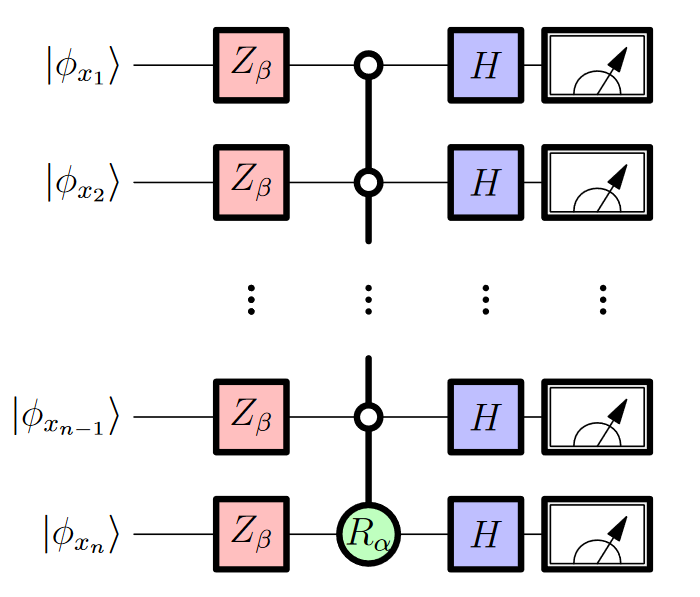
\includegraphics[scale =1]{measurement}\end{tikzfigure}}
            \subcolumn{0.4}
                \block{}{\begin{tikzfigure}[Plot of $f_{n}(\beta)$ where $\theta$ is apporopriately bounded]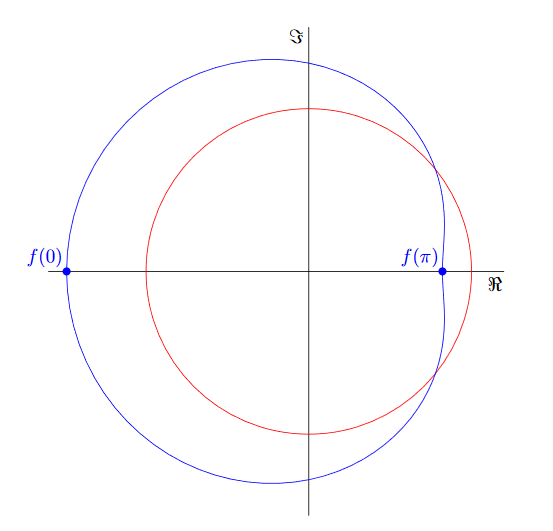
\includegraphics[scale = 0.75]{function}\end{tikzfigure}}
                \end{subcolumns}
            \block{Noise tolerance}{This argument can also be made noise tolerant. If $\Lambda$ is the space of values for $\lambda$ and $\mu_{i}(\lambda)$ gives the probability distribution that a preparation methods assigns for the physical state of $\ket{\phi_{i}}$ then the total variation distance defined by $$D(\mu_{0},\mu_{1}) = \int_{\Lambda}\left |\mu_{0}(\lambda)-\mu_{1}(\lambda) \right  |d\lambda $$ determines how distinguishable the two distributions are. It can be shown that $D \leq 1 - \sqrt[n]{\epsilon}$ where $\epsilon$ is the maximum distance between probabilities measured in the lab and those predicted by QM. So as we make $\epsilon$ small the distributions become increasingly distinct i.e.  $\lambda$ cannot agree with both states. }
            \block{}{\small Mathew F. Pusey, Jonathon Barrett, Terry Rudolph. The quantum states cannot be interpreted statistically. Poster presented at University of Melbourne PHYC30018 2018 poster session.}
        \column{0.6}
            \block{The difference}{Let $\lambda$ be the set of all physical properties of a system. The statistical view holds that $\lambda$ can be in agreement with more than one state vector, although given a certain $\lambda$ one state could be more likely than the other. If, on the other hand, the quantum state is a physical property then $\lambda$ uniquely determines the quantum state of a system.}
            \block{General approach}{Suppose by way of contradiction that the statistical view is correct. Consider then two preparation methods such that one prepares the pure state $\ket{\phi_{0}}$ and the other $\ket{\phi_{1}}$. Prepare $n$ states such that their physical states are uncorrelated. Then there is probability $p > 0$ that the physical state $\lambda_{i}$ of each system agrees with both methods of preparation \\ $\Rightarrow$ there is a probability $q^{n} > 0$ that the physical state of the combined system of $n$ particles is compatible with every one of the $2^{n}$ possible states. Now if a joint measurement procedure could be devised such that each outcome has probability zero given one of the $2^{n}$ states then we have arrived at the desired contradiction, since, in such a case, the measurement apparatus would be uncertain of the preparation method used $q^{n}>0$ portion of the time and hence would run the risk of returning an outcome that quantum mechanics predicts should occur with probability zero. We must now fix $n$ and also devise this measurement procedure}
           \block{Measurement}{Given any two distinct states we can pick a basis of the Hilbert space such that $$\ket{\phi_{0}}= \cos\frac{\theta}{2}\ket{0} + \sin\frac{\theta}{2}\ket{1}, \hspace{0.5cm} \ket{\phi_{1}}= \cos\frac{\theta}{2}\ket{0} - \sin\frac{\theta}{2}\ket{1} $$ with $0 \leq \theta \leq \pi/2$. We can then treat these as qubits w.l.o.g. By restricting our attention to the subspace spanned by these two states. Prepare $n$ systems such that the total state is $\ket{\phi_{x_{1}}}\bigotimes \ket{\phi_{x_{2}}}\dots \bigotimes \ket{\phi_{x_{n}}} \equiv \ket{x_{1}x_{2}\dots x_{n}}$ where $x_{i} = 0 (1)$ if the $i^{th}$ system is prepared in the $\ket{\phi_{0}} (\ket{\phi_{1}})$ state. Now the measurement procedure consists of a series of quantum logic gates applied to every state followed by a measurement of each system in the basis $\{\ket{0},\ket{1}\}$. The gates are applied as indicated in Fig. 1 and they are defined as follows: $$H = \frac{1}{\sqrt{2}}\begin{pmatrix}1 && 1 \\ 1 && -1\end{pmatrix}, \hspace{0.5cm} Z_{\beta} = \begin{pmatrix}1 && 0 \\ 0 && e^{i\beta}\end{pmatrix}$$ and $R_{\alpha}\ket{00\dots0} = e^{i\alpha}\ket{00\dots0}$. $R_{\alpha}$ acts as the identity on all other states.  Then the probability of each measurement $\bra{x_{1}x_{2}\dots x_{n}}$ outcome is given by the squared absolute value of {\small$$\bra{x_{1}x_{2}\dots x_{n}}H^{\bigotimes n}R_{\alpha}Z^{\bigotimes n}\ket{\phi_{x_{1}}}\bigotimes\ket{\phi_{x_{2}}}\dots \bigotimes \ket{\phi_{x_{n}}} \propto e^{i\alpha}+(1+e^{i\beta}\tan \frac{\theta}{2})^{n}-1 = e^{i\alpha} - f_{n}(\beta) $$} $f_{n}(\beta)$ is shown for $2\arctan(2^{1/n}-1) \leq \theta \leq \pi/2 $ in Fig. 2 and since it crosses the unit circle then the RHS of the above has a solution for some $\beta$. This also gives us a lower bound on $n$ and so we're home!}




    \end{columns}
\end{document}
